\documentclass[tikz,border=8pt]{standalone}
% Shared look for every TikZ diagram. Load with \input{../../tools/tikz-style.tex}
\usepackage[T1]{fontenc}
\usepackage{lmodern}
\renewcommand{\sfdefault}{lmr}  % diagrams use the same serif as the text
\usetikzlibrary{arrows.meta, positioning, shapes.geometric, calc, fit, backgrounds}
\definecolor{cblue}{HTML}{4C78A8}
\definecolor{corange}{HTML}{F58518}
\definecolor{cgreen}{HTML}{54A24B}
\definecolor{cred}{HTML}{E45756}
\definecolor{cpurple}{HTML}{B279A2}
\definecolor{cgrey}{HTML}{6B6B6B}
\tikzset{
  every picture/.style={font=\sffamily, line width=1.2pt},
  box/.style={draw=#1, fill=#1!12, rounded corners=4pt, align=center, inner sep=7pt, minimum height=1.1cm},
  box/.default=cgrey,
  arrow/.style={-{Stealth[length=3mm]}, draw=cgrey, line width=1.4pt},
  title/.style={font=\sffamily\bfseries\Large},
  note/.style={font=\sffamily\small, text=cgrey, align=center},
}
\AtBeginDocument{\hyphenpenalty=10000 \exhyphenpenalty=10000}

\begin{document}
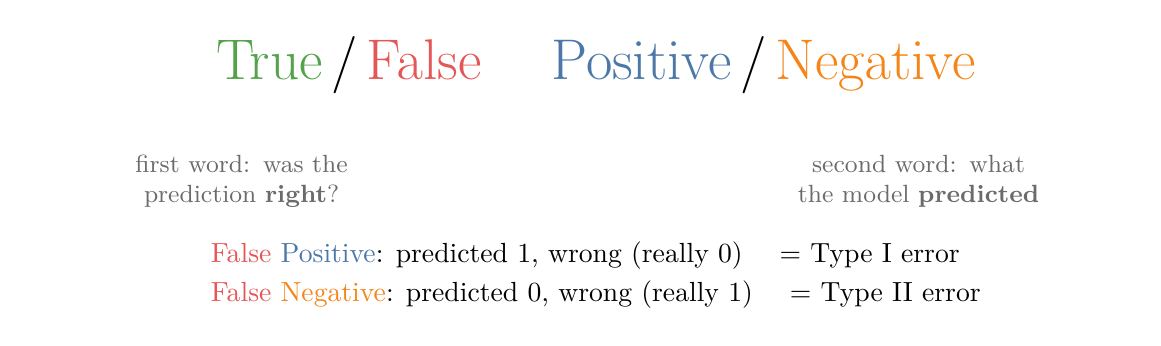
\begin{tikzpicture}
  \node[font=\huge] (w) {\textcolor{cgreen}{True}\,/\,\textcolor{cred}{False} \quad \textcolor{cblue}{Positive}\,/\,\textcolor{corange}{Negative}};
  \node[note, text width=5.2cm, below left=0.5cm and -3.2cm of w] (a) {first word: was the prediction \textbf{right}?};
  \node[note, text width=5.2cm, below right=0.5cm and -3.6cm of w] (b) {second word: what the model \textbf{predicted}};
  \node[below=1.6cm of w, align=left] (ex) {%
    \textcolor{cred}{False} \textcolor{cblue}{Positive}: predicted 1, wrong (really 0) \quad = Type I error\\[2pt]
    \textcolor{cred}{False} \textcolor{corange}{Negative}: predicted 0, wrong (really 1) \quad = Type II error};
\end{tikzpicture}
\end{document}
